\section{Heuristics approaches for pairwise sequence alignment}
These methods are very popular because they are much faster than dynamic
programming and at the same time they return excellent alignment of biologica
sequences.

\subsection{General strategy}

The general strategy of these methods is based on two main steps:
\begin{enumerate}
  \item Produce a lookup table where the words of length $k$ (k-mers) present
in sequence A are indexed, including all the position where they occur in
sequence A.
  \item Read sequence B, word by word. For every word check in the lookup talbe
if and where the word occur in sequence A. Then try to extend the alignment.
\end{enumerate}

Other strategies are: FASTA, BLAST and BLAT.

\paragraph*{Conversion of DNA kmerso into numbers}

With a given DNA you can translate ACGT with a binary number. In this way you
can convert a DNA sequence into a number. This can be done also with ammino
acid.
But how do you fill up the metrics? This is why there are different metrics.

\subsection{FASTA}

Imagine a sequence placed at the top and a sequence placed on the left side,
both starting at the top left corner. The sequence at the top is indexed,
memoriing all the occurrences and position ofeach kmer. Then the sequence at
the left is read, one kmer at a time. All the "growing" diagonals are memorized
to produce the result shown in panel A.

For example, if you have kmer of length one ($ktup = 1$), you will find better
performance in confront of Smith \& Waterman. This because you have to do less
operation with FASTA.

You use Smith \& Waterman only if you go for a full match, because analize a
full alignment it's expensive but Smith \& Waterman it's more accurate.

\begin{figure}[H]
  \centering
  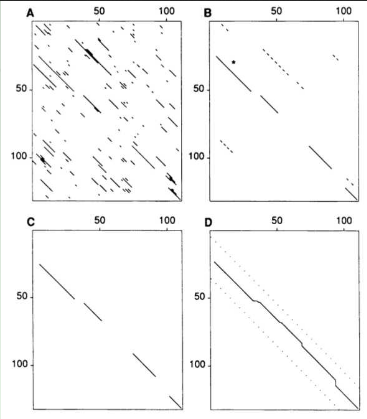
\includegraphics[scale=0.5]{FASTA}
  \caption{FASTA}
\end{figure}

Question: If I have a very long sequence and several short DNA sequence, is it
better to index the long or the short sequence? Reply: it's better to index
the long database, because you can check all the differents sequence in the
database where are all the data.

\subsection{BLAST}

Blast is probably the most popular program for the alignment of biological
sequences.

As the other, also BLAST use a lookup table, but it create also one for the
similarities with a given threshold. Another difference from FASTA is that
BLAST tries to extend locally each "seed", to obtain a High-scoring segment
pair.

\begin{figure}[H]
  \centering
  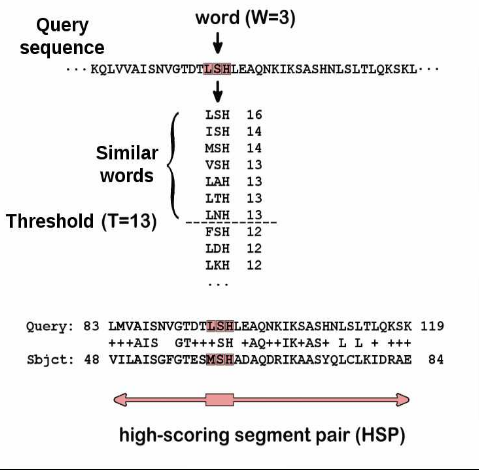
\includegraphics[scale=0.5]{BLAST}
  \caption{BLAST}
\end{figure}

BLAST it's little faster than FASTA. Most people use BLAST also for DNA
alignment and it works well.

Different flavours of BLAST:
\begin{itemize}
  \item Nucleotide blast
  \item Protein blast
  \item blastx
  \item tblastn
  \item tblastx
\end{itemize}

%exam question
What's the sense of translate the sequence in proteins? If you consider
evolution of sequences, the natural selection is keepeng some of this
information working and very often this natual selection it's working at the
protein level. So sometime you can have 2 nucleotide sequences completely
different but that encode the same protein. So it's much more accurate do it at
the protein level.

\subsection{BLAT}

BLAT is an alignment tool like BLAST, but it's structured differently. On DNA,
BLAT works by keeping an index of an entire genome in memory.

The best things to do it's to align RNA with Genom.

New version of BLAT can index more kmer.
